\PassOptionsToPackage{pdfpagelabels=false}{hyperref} 
\documentclass{sigchi}

% Use this command to override the default ACM copyright statement
% (e.g. for preprints).  Consult the conference website for the
% camera-ready copyright statement.

%% EXAMPLE BEGIN -- HOW TO OVERRIDE THE DEFAULT COPYRIGHT STRIP -- (July 22, 2013 - Paul Baumann)
% \toappear{Permission to make digital or hard copies of all or part of this work for personal or classroom use is      granted without fee provided that copies are not made or distributed for profit or commercial advantage and that copies bear this notice and the full citation on the first page. Copyrights for components of this work owned by others than ACM must be honored. Abstracting with credit is permitted. To copy otherwise, or republish, to post on servers or to redistribute to lists, requires prior specific permission and/or a fee. Request permissions from permissions@acm.org. \\
% {\emph{CHI'14}}, April 26--May 1, 2014, Toronto, Canada. \\
% Copyright \copyright~2014 ACM ISBN/14/04...\$15.00. \\
% DOI string from ACM form confirmation}
%% EXAMPLE END -- HOW TO OVERRIDE THE DEFAULT COPYRIGHT STRIP -- (July 22, 2013 - Paul Baumann)

% Arabic page numbers for submission.  Remove this line to eliminate
% page numbers for the camera ready copy
\pagenumbering{arabic}

% Load basic packages
\usepackage{balance}  % to better equalize the last page
\usepackage{graphics} % for EPS, load graphicx instead 
\usepackage[T1]{fontenc}
\usepackage{txfonts}
\usepackage{mathptmx}
\usepackage{pgfplots}
\usepackage{pgf-pie}
\usepackage{tikz}
\usepackage{environ}
\usepackage{tikzscale}
\usepackage{comment}
\usepackage{amssymb}
\usepackage{wrapfig}
\usepackage{booktabs}
\usepackage{framed}


\usepackage{subcaption}

\usepackage{verbatim}


\pgfplotsset{compat=1.8}
\usepgfplotslibrary{statistics}


\usepackage[pdftex]{hyperref}
\usepackage{color}
\usepackage{booktabs}
\usepackage{textcomp}
% Some optional stuff you might like/need.
\usepackage{microtype} % Improved Tracking and Kerning
% \usepackage[all]{hypcap}  % Fixes bug in hyperref caption linking
\usepackage{ccicons}  % Cite your images correctly!
% \usepackage[utf8]{inputenc} % for a UTF8 editor only

% If you want to use todo notes, marginpars etc. during creation of your draft document, you
% have to enable the "chi_draft" option for the document class. To do this, change the very first
% line to: "\documentclass[chi_draft]{sigchi}". You can then place todo notes by using the "\todo{...}"
% command. Make sure to disable the draft option again before submitting your final document.
\usepackage{todonotes}

% Paper metadata (use plain text, for PDF inclusion and later
% re-using, if desired).  Use \emtpyauthor when submitting for review
% so you remain anonymous.
\def\plaintitle{Slide: Fast Text Entry for Virtual Reality}
\def\plainauthor{First Author, Second Author, Third Author,
  Fourth Author, Fifth Author, Sixth Author}
\def\emptyauthor{}
\def\plainkeywords{virtual reality; text input; text entry; multimodal.}
\def\plaingeneralterms{Documentation, Standardization}

% llt: Define a global style for URLs, rather that the default one
\makeatletter
\def\url@leostyle{%
  \@ifundefined{selectfont}{
    \def\UrlFont{\sf}
  }{
    \def\UrlFont{\small\bf\ttfamily}
  }}
\makeatother
\urlstyle{leo}

% To make various LaTeX processors do the right thing with page size.
\def\pprw{8.5in}
\def\pprh{11in}
\special{papersize=\pprw,\pprh}
\setlength{\paperwidth}{\pprw}
\setlength{\paperheight}{\pprh}
\setlength{\pdfpagewidth}{\pprw}
\setlength{\pdfpageheight}{\pprh}

% Make sure hyperref comes last of your loaded packages, to give it a
% fighting chance of not being over-written, since its job is to
% redefine many LaTeX commands.
\definecolor{linkColor}{RGB}{6,125,233}
\hypersetup{%
  pdftitle={\plaintitle},
% Use \plainauthor for final version.
%  pdfauthor={\plainauthor},
  pdfauthor={\emptyauthor},
  pdfkeywords={\plainkeywords},
  bookmarksnumbered,
  pdfstartview={FitH},
  colorlinks,
  citecolor=black,
  filecolor=black,
  linkcolor=black,
  urlcolor=linkColor,
  breaklinks=true,
}

% create a shortcut to typeset table headings
% \newcommand\tabhead[1]{\small\textbf{#1}}

% End of preamble. Here it comes the document.
\begin{document}

\title{\plaintitle}
\def\emptyauthor{}
\begin{comment}
\numberofauthors{3}
\author{%
  \alignauthor{Leave Authors Anonymous\\
    \affaddr{for Submission}\\
    \affaddr{City, Country}\\
    \email{e-mail address}}\\
  \alignauthor{Leave Authors Anonymous\\
    \affaddr{for Submission}\\
    \affaddr{City, Country}\\
    \email{e-mail address}}\\
  \alignauthor{Leave Authors Anonymous\\
    \affaddr{for Submission}\\
    \affaddr{City, Country}\\
    \email{e-mail address}}\\
}
\end{comment}
\maketitle

\begin{abstract}
The lack of proprioception makes it challenging for users to use a real keyboard in virtual reality.
This paper proposes SwipeVR, a virtual keyboard that requires only a trackpad, which are available in existing VR input devices today.  The key design principles underlying SwipeVR are: (1) Relative positioning: the user's finger is pointing to the same position in a keyboard upon first contact.
(2) Keybatching with smart correction: the keyboard is partitioned into 8 tiles.  The user does not have to hit the right key, but just the tile that contains the key.
(3) Intention-based mixed keyboard.  The user can also type on the full keyboard - the intent in the choice of the batched vs full keyboard is automatically inferred.
This paper performs a user study across the various design choices as well as existing input methods.
We found that SwipeVR is easy to learn and provides a similar speed to text entry on a mobile phone keyboard.



We present what we believe is the most efficient and fastest text entry method available for virtual reality.
SwipeVR strives for simplicity while maintaining good performance.
For full words, the user gestures on the touch pad of the controller wand to a sector of the keyboard.
Full access to characters, punctuation, and digits are accessible through a secondary keyboard.
Error correction and editing are supported with multi-wand gestures.
The system is able to be learned quickly by beginners and supports eyes-free entry by experts.
The effort to enter text is comparable to gesture text entry on a mobile phone.
We conduct a study with X participants where an average text entry speed of Y WPM was observed with an error rate of Z\%.  
These results show that text entry is similar to that of a mobile phone keyboard but error correction and editing, the most time consuming step, is greatly improved.




\end{abstract}

\category{H.5.1.}
{Information Interfaces and Presentation (e.g. HCI)}
{Multimedia Information Systems}
\category{I.3.7.}
{Computer Graphics}
{Three-Dimensional Graphics and Realism}

%link at: http://www.acm.org/about/class/ccs98-html

\keywords{\plainkeywords}



\section{Introduction}

While the primary use of virtual reality is in games and videos today, it can be used in many application domains, from education, architectural reviews~\cite{guerreiro2014beyond}, healthcare, large group chats ~\cite{mcnerney1999system}, and data visualization~\cite{abbott2011empire}, exploration of space and other dangerous locations, scientific visualization, manufacturing, journalism, traveling, architecture, shopping.

Today's commercial virtual reality systems have relatively primitive input devices.
The most advanced controller available are the hand-tracked controllers provided by HTC Vive.
They enable users to interact with the objects in the virtual space, and it includes a trigger and a trackpad style click wheel.
The Oculus Rift currently uses a game controller, and the Samsung Gear has a couple of buttons on the headset.

This paper studies a very basic form of input in virtual reality environments: text.  There are many uses of text input in virtual reality, from typing in account names, passwords, search items, people you wish to contact, writing notes and chatting with others.    

The average typing performance on a regular keyboard was found to be about 60 words per minute\cite{Varcholik}, thanks to the dexterity of our fingers, the haptic feedback from the physical keyboards, and visual feedback on the display.    In the context of virtual reality, it is often not an option to use a physical keyboard.  We are usually not sitting down and it is hard to switch between the VR controllers and a physical keyboard, further complicated by the fact that we cannot see the keyboard in VR. It is desirable to be able to type with existing VR input devices, so we do not have to remove the head gear to type. 

Typing is challenging in virtual reality because of the latency in visual feedback and the lack of proprioception.  The industry standard is to enter text with gaze.  A virtual keyboard is presented in VR, and users type a letter by gazing at the desired key and tapping on the gear or controller.  Not only did the users find the process slow, but it can also causes nausea as they tap the head gear.  The user can type about 7 words per second.   

Entering text via speech is attractive, especially in the immersive virtual reality environment.   However, speech recognition is limited when typing passwords, names, and URLs~\cite{TODO}. 
The lack of user acceptance is also due to issues such as privacy, the perception of bothering others, the awkwardness of speaking to a machine~\cite{sawhney2000nomadic}.
Some users find voice as unreliable especially when the accent or ambient sound negatively affect accuracy.
Other alternatives proposed including using gesture, motion controllers, Leap Motion or tangibles, handheld controllers, or relying on a subset of keyboard and mouse commands~\cite{billinghurst1999collaborative}.
All these existing solutions, while potentially good for simple tasks, aren't adequate for tasks that requires a greater bandwidth of input~\cite{McGill:2015:DRO:2702123.2702382}.

For those situations where speech input is unacceptable, it is desirable to be able to enter text simply, quickly, and accurately on a touchpad, which is already built into the Vive controllers.   

\subsection{Informal Studies}
We started our research by trying some  possibilities.
\begin{enumerate}
\item
Gazing.  Users enter keys by gazing at the keys in a virtual keyboard. 

\item

Drumming.  One proposal is to display the keys as a virtual drum kit, and users enter keys by hitting the corresponding drums using the controllers as drumsticks. 

\item
Augmented reality.  We let users see their fingers and touchpad by streaming the view through a camera into virtual reality.  

\item
26-key tapping.  Users tap on the soft keyboard on the touchpad is shown as a virtual keyboard in virtual reality.   The users can see the keys being touched in the keyboard, as well as the words being type in a textbox.

\item
26-key swiping.  Users swipe on the soft keyboard on the touchpad instead.  
\end{enumerate}

The typing speed that we observed in these trials were in the range of 10-15 words per minute, far below our target performance.  Our initial trials reveal the deficiencies in each of these approaches.

\subsection{Contributions}
This paper proposes the Slide virtual keyboard, which uses three main design concepts: 
\begin{enumerate}
\item
Self-relative vectors.  To enter a character, the user slides from what is assumed to be the centroid of the keyboard to the key of interest.  

\item
Directional input, with error correction.  All keys are grouped in 6 tiles, and the user only has to slide in the direction of the tile containing the key.  A Bayesian word recommender determines the word entered. 

\item
Intention-based hybrid keyboard: the keyboard automatically switches between the 26-key and 6-tile keyboard based on the user's finger movements.  
\end{enumerate}

Our experiments show that …

In contrast, a recent study shows an average of 53 words per minute when typing on mobile devices\cite{landay}.


\section{Related Work}

In this section, we discuss studies applicable to virtual reality based text entry.
For a full review of text entry methods, see~\cite{mackenzie2002text, zhai2005search, Buxton2011}.

\subsection{Novel QWERTY Keyboards}
Researchers have leveraged a users' familiarity with the QUERTY~\cite{noyes1983qwerty} keyboard to make their novel devices easier to use.
The Half-QWERTY keyboard~\cite{matias1993half} is arm-mounted and has a reduced size by using only half of a QWERTY keyboard.
The Pinch Gloves~\cite{bowman2002text} controls a virtual keyboard with hand rotations and finger-mounted buttons.
Another glove, KITTY~\cite{Kuester:2005:TKI:1101616.1101635} uses the tapping of contacts on each finger with the thumb to mimic a keyboard.
DigiTap~\cite{Pratorius:2014:DEV:2671015.2671029} is a similar idea but uses a wrist mounted camera instead of a glove.

\subsection{Word Gesture Keyboards}
Word gesture keyboards such as ShapeWriter~\cite{zhai2012word,Zhai:2009:SIL:1520340.1520380} and SHARK 2~\cite{kristensson2004shark}, are gesture based text input methods.
Words are written through a gesture that links the letters of the intended word on a soft keyboard. A language model and word prediction is required to select the most likely word from  candidate words.
For out of vocabulary and hard-to-predict words, a deterministic input method is still needed.
VelociTap~\cite{vertanen2015velocitap} takes the predictive model further by only predicting the whole sentence.

\subsection{Gloves and Chording Keyboards}
Other approaches abandon the QWERTY keyboard entirety.
Chording keyboards~\cite{noyes1983chord}, such as Twiddler~\cite{lyons2004twiddler} use a combination of a few keys to produce characters.
Chording is done is done with gloves, such as Chording Glove~\cite{rosenberg1999chording}.
The VirtualPhonepad~\cite{ahn2006virtualphonepad} imitates text entry via a $3\times3$ mobile phone keypad.
Virtual Notepad~\cite{poupyrev1998virtual} allows for creating handwritten annotations in virtual reality.
Connecting the Dots~\cite{frees2006connecting} approximates handwriting by having users connect dots on a $3\times3$ virtual dot matrix to scribe a single character.

In a literature review, the Pinch Gloves, pen and tablet, chording keyboard, and a speech-based are compared~\cite{bowman2002text}.
The pen and tablet and speech are fastest.  The pen and tablet had the fewest errors.
The comparison was done before specialized virtual reality input device were invented.

\subsection{Home Entertainment Input Devices}
Text entry methods is sought after in other application areas, such as home entertainment systems.
SpeeG~\cite{hoste2012speeg} is a Kinect~\cite{geerse2015kinematic} version of Speech Dasher~\cite{vertanen2010speech} text input technique.
The user speaks and then corrects mistakes using an interface that scrolls through the recognized text as well as alternatives.
SpeeG2~\cite{hoste2013speeg2} uses a grid instead of a scroll.

\subsection{Speech recognition}
Spoken language is effective for human-human interaction but often has severe limitations when applied to human-computer interaction.
Speech is slow for presenting information and interferes significantly with other cognitive tasks~\cite{shneiderman2000limits}.

Speech recognition is limited when typing passwords, names, and URLs~\cite{TODO}. 
The lack of user acceptance is also due to issues such as privacy, the perception of bothering others, the awkwardness of speaking to a machine~\cite{sawhney2000nomadic}.
Some users find voice as unreliable especially when the accent or ambient sound negatively affect accuracy.
Studies have shown that users find it ``harder to talk and think than type and think" and considered the keyboard to be more ``natural" than speech for text entry ~\cite{Karat:1999:PEC:302979.303160}.

In virtual reality, a Japanese speech-based entry system represents candidate words recognized by the speech recognition engine as blocks that can be moved around in the virtual enviroment~\cite{osawa2002multimodal}. 

For mobile phones, speech entry is three times faster than typing for English and Mandarin~\cite{ruan2016speech}.  
In this experimental setup, participants were given a set of phrases to type and speak.
The phrases are given ahead of time, but normal speech is filled with hesitations, repetitions, changes of subject in the middle of an utterance~\cite{forsberg2003speech} as the user thinks.
This could lead to an unrealistic accuracy for speech.  
The study also excludes punctuation marks and capital letters from the phrases.
Generating accurate punctuation  automatically with speech input is not yet possible and must be done manually~\cite{chen1999speech}.

\subsection{Gaze Directed Typing}
Gaze directed typing is the main text input method used today in systems such as Oculus G earVR. A main advantage of this method is that it uses the available hardware and does not require an additional device. This method is slow~\cite{card1983psychology, mackenzie1992fitts} and inconvenient since the whole head has to be moved for each character.
Moving the head while the VR scene remains static also often causes nausea or dizziness~\cite{atienza2016interaction}.   

\subsection{Text Input with Virtual Reality Controllers}
While early, input methods and controllers are being developed specifically for use in virtual reality.
FaceTouch~\cite{Gugenheimer:2016:FTI:2851581.2890242} has the backside of the head mounted display that as a touch sensitive surface.
The user selects virtual content by touching the corresponding location on backside of the display.
It is useful but only for short periods of time before the users' arms get tired.

Belt~\cite{dobbelstein2015belt} is a novel unobtrusive input device for wearable displays that has a touch surface encircling a users' hip.
The wide input space for a horizontal spatial mapping but suffers from low throughput, arm fatigue, and social acceptance.
Nenya~\cite{ashbrook2011nenya} uses a finger ring as an input mechanism that is always available.
It is fast to access, allows analog input, and is socially acceptable by being embodied in a commonly worn item.

Industry has started to standardize around a virtual reality controller.  HTC, Facebook, and Google have all released a virtual reality hardware design.
Each includes a controller, shown in Figure~~\ref{fig:controllers}.
They all similar in the they all contain a rotational tracking, a way to track the thumb through either joystick or touchpad, and at least four buttons.
Vive and Oculus use an absolute tracking system to minimizing sensor drift and to allow for rotational and translational tracking~\cite{hilfert2016low}.
The Daydream controller, shown in Figure~\ref{fig:controllerDaydream}, in only for a single hand whereas the others have a controller for each hand.
SwipeVR is implemented using the Vive but could be implemented on the other two.

\newcommand{\ra}[1]{\renewcommand{\arraystretch}{#1}}


\begin{table*}\centering
\ra{1.3}
\begin{tabular}{@{}rrrrrr@{}}\toprule
						& $Speech$ 		& $Gaze$ 		& $Mobile$		& $SwipeVR$  \\
\midrule
$Positioning$			&				& absolute		& absolute		& relative	  		\\
$Hardware$ 				&microphone 	& HMD \& button	& touch screen	& controller		\\
$Keys$ 					&				& 26+			& 26+			& 6					\\
$Special~Characters$ 	&				& \checkmark	& \checkmark	& \checkmark		\\
$Granulatiry$ 			&word			& character		& character		& word or character	\\
$Hands$ 				& 0				& 1				& 1 or 2		& 1					\\
$Real-Time~Feedback$ 	& word			& character		& character		& word				\\
$Cursor~Mode$ 			& NA			& persistent	& NA			& snap-to-home		\\
$Silent$ 				&				& \checkmark	& \checkmark	&\checkmark			\\
$Muscle$ 				& vocal chords	& neck			& fingers		& thumb			\\
$WPM$					& \%\cite{sppechTBA} & \%		& \%			& \%\\
$Error~Rate$			& \%\cite{sppechTBA} & \%		& \%			& \%\\

%    Correction Method		& X 			& X 			& X				& 	\checkmark		\\ 

\bottomrule
\end{tabular}
\caption{Ontology of input methods.}
\label{table:ontology}
\end{table*}

\begin{figure}
  \centering
	\begin{subfigure}{.4\columnwidth}
  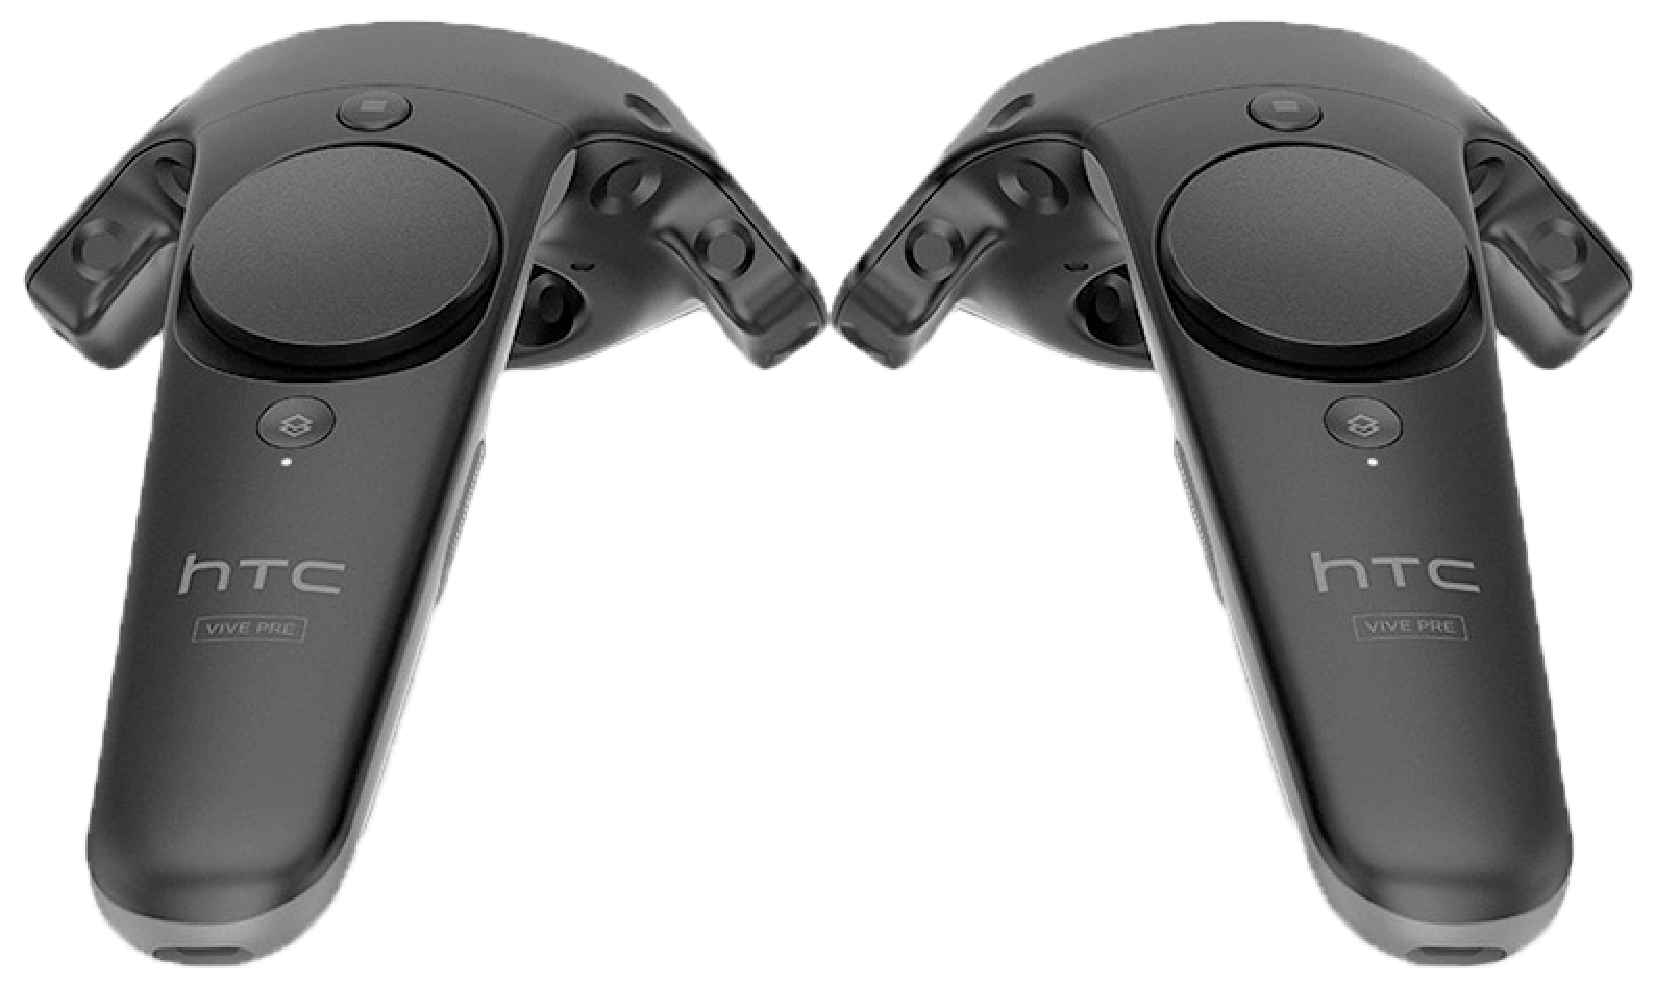
\includegraphics[width=\textwidth]{figures/controllerVive}
  \caption{HTC's Vive }\label{fig:controllerVive}
  \end{subfigure}
  \\
  \begin{subfigure}{.4\columnwidth}
  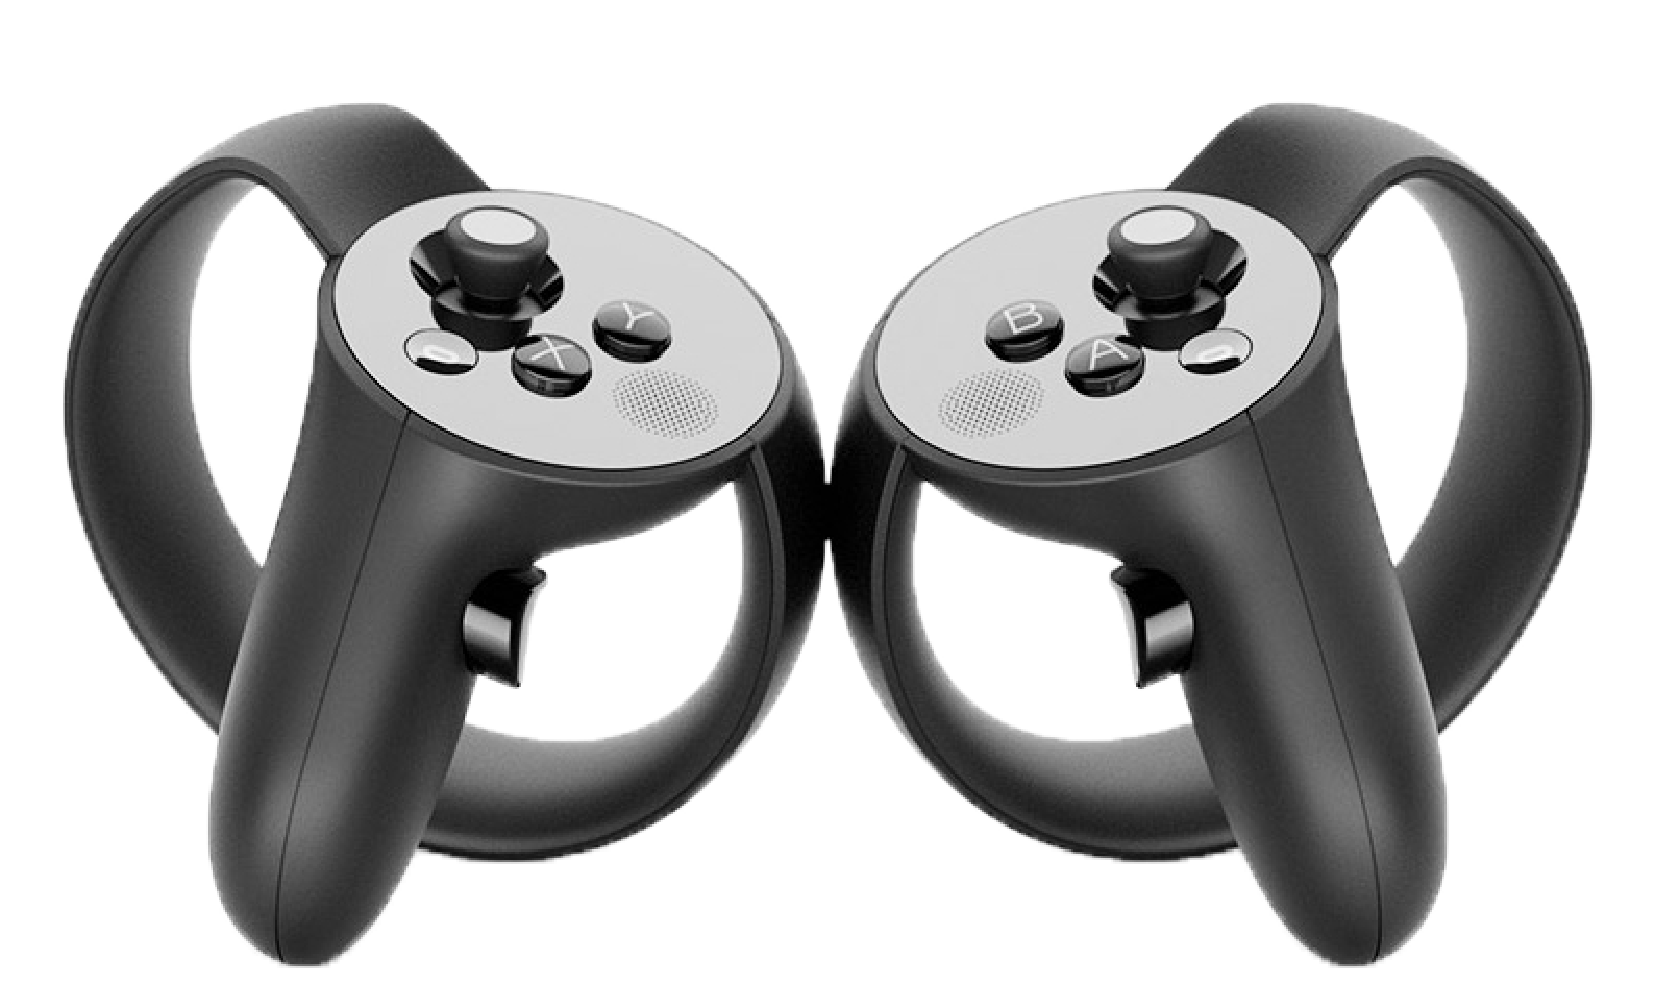
\includegraphics[width=\textwidth]{figures/controllerOculus}
  \caption{Facebook's Oculus}\label{fig:controllerOculus}
  \end{subfigure}
  \\
  \begin{subfigure}{.4\columnwidth}
  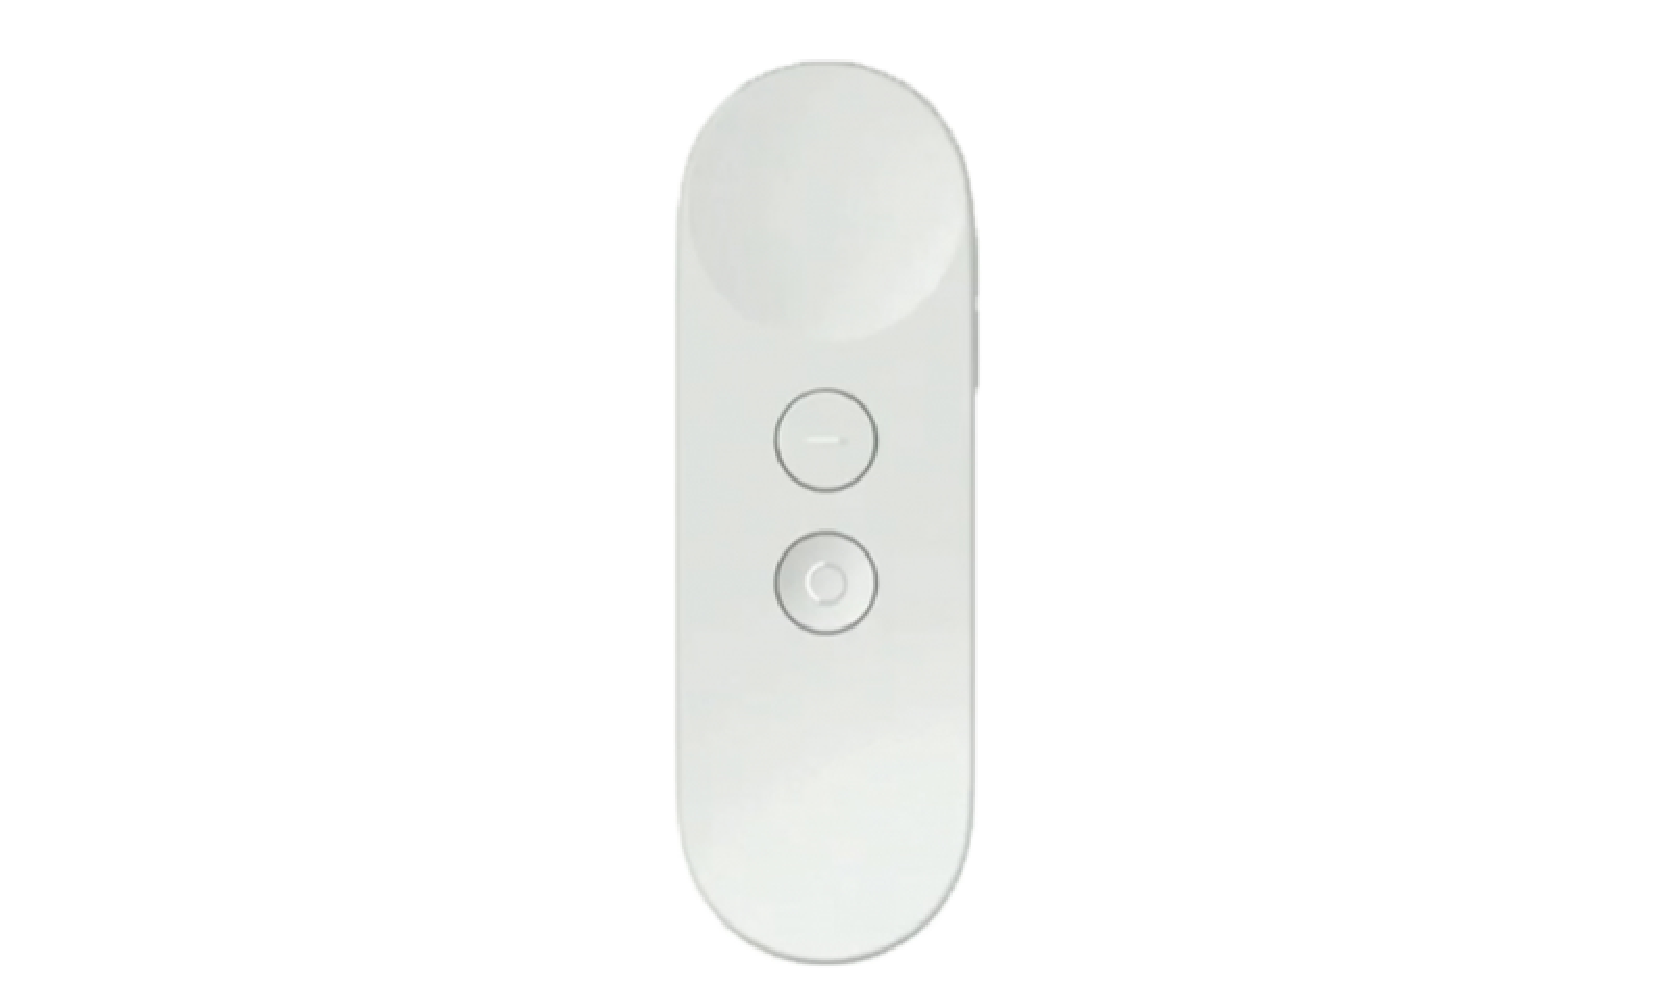
\includegraphics[width=\textwidth]{figures/controllerDaydream}
  \caption{Google's Daydream}\label{fig:controllerDaydream}
  \end{subfigure}
  \caption{
  Industry is standardizing on some of the important components for virtual reality controllers.
  The three major controllers shown above all contain a way to track the thumb, at least 3 degrees of freedom tracking  (rotational), and at least four buttons.
  The Vive (\subref{fig:controllerVive}) and the Oculus (\subref{fig:controllerOculus}) use room-scale tracking to give 6 degrees of freedom (rotation and translation).  
  Many virtual reality systems today are released with a controller for each hand.  
  The Vive and Daydream (\subref{fig:controllerDaydream}) employ a thumb track pad to capture finger movement.
  Oculus controller uses joysticks instead.
  The system described in this paper is implemented using the Vive and could be implemented on the other two.
  }~\label{fig:controllers}

\end{figure}




\section{Challenges of Text Entry in Virtual Reality}
Text entry is a  an extreme use in testing our ability to interact between the physical and virtual world.

\subsection{Latency}
Typing is complex interaction that requires a high-bandwidth feedback loop~\cite{McGill:2015:DRO:2702123.2702382}.
Latency is a barrier in achieving a seamless interaction between the real and virtual~\cite{leedesigning}.

In virtual reality, latency is the time between movement of the user's head and the updated image being displayed on the screen.  
This includes time includes the times for fusion, image transmission,
rendering, sensor response and display response.
This is commonly referred to as the \textit{motion-to-photon} latency.

To achieve a genuine sense of presence~\cite{schuemie2001research} in virtual reality, the total \textit{motion-to-photon} latency must be less than 20 milliseconds~\cite{jerald2009relating,jerald2010scene,bailey2004latency} for head movement.
Some existing systems have a latency as high as 80 milliseconds ~\cite{lincoln2016motion,dallaire2016animated}.

Touch-based interactions need even tighter tolerances on latency compared to head movement described above.
Research on touchscreens finds that for a user to perceive display elements as naturally being affected by touch, there is a perceptual floor between 2  and 11 milliseconds below which users do not notice lag~\cite{Jota:2013:FFE:2470654.2481317,Ng:2012:DLD:2380116.2380174}.

Further, they find that latencies down to 2.38 milliseconds are required to alleviate user perception when dragging~\cite{Jota:2013:FFE:2470654.2481317,Ng:2012:DLD:2380116.2380174}.

\subsection{Reduced Precision}
Haptic feedback and physical constraints in real world input devices help to define interactions. 
Fine-grained control is difficult in in virtual reality and restricts users to the coarse manipulation of virtual objects.
Input device that excluded the use of the fingers are slower~\cite{Zhai:1996:IMG:238386.238534}.

\subsection{Limited Proprioception}
Manipulation in virtual reality is difficult because users must do without the haptic contact with keyboard buttons they rely on in the real world to orient themselves.
To compensate for this, we propose using relative instead of absolute positioning for entry.


\section{Design Goals}
Before describing the prototypes and lessons learned, we present five high-level design goals that focus on input metrics, user experience, and adaptability.
These goals are informed by related work and our experience building other systems.

\subsection{Efficient}
How closely does the new device approach exceed the speed of the best devices for text input in virtual reality?

\subsection{Learnable}
How long does the device take to learn?
Does it rely on existing skills?
Is there ways for the user to transition from being a novice to an expert?

\subsection{Practical}
Is the input method usable today?
Moreover, will it be usable in the future given the where we think virtual reality controller are heading?

\subsection{General}
Is the text input method useful across multiple types of applications?
Can the user type their username, password, and a message to a friend?

\subsection{Usable}
Desktop user sessions are longer than mobile~\cite{Kamvar:2009:CIM:1526709.1526817}.
We hypothesize that virtual reality will have a user session time closer to that of a desktop computer than a mobile phone.
Once a user has take the time to wear the head mounted display and controller, the session will
Midair interactions are prone to fatigue and lead to a feeling
of heaviness in the upper limbs~\cite{Hincapie-Ramos:2014:CEM:2556288.2557130}, commonly known as the \textit{gorilla arm effect}.
Will the user be able to use the text input method comfortably?
Can they use it for as long as they use as they their computer at night?

\section{Prototyping Process}
During the prototyping process, we ask a users to type a few sentences using the input device. 
The users was given little to no instruction about how the input device worked.
The goals of this process was to explore the performance potential of each input device and to investigate if users could understand the visual interface.
We record how long the input took, their understanding of the input device, and their other feedback.

\subsection{Design \#1 - External Camera}
\vspace*{.1cm}

\includegraphics[width=.9\columnwidth]{figures/sigchi-logo}

For the first pilot, we build a prototype that streams from the front facing camera on the head mounted display into the virtual enviroment.
The camera is pointed at a soft mobile keyboard.
The goals of this pilot is to investigate how latency and presence, particular of the fingers, affect performance.
Latency is an inhibitor to fast input.
Additionally, muscle memory is not as accurate as we expect and drifts quickly after a few taps.

\subsection{Design \#2 - 26-key Tap}
\vspace*{.1cm}
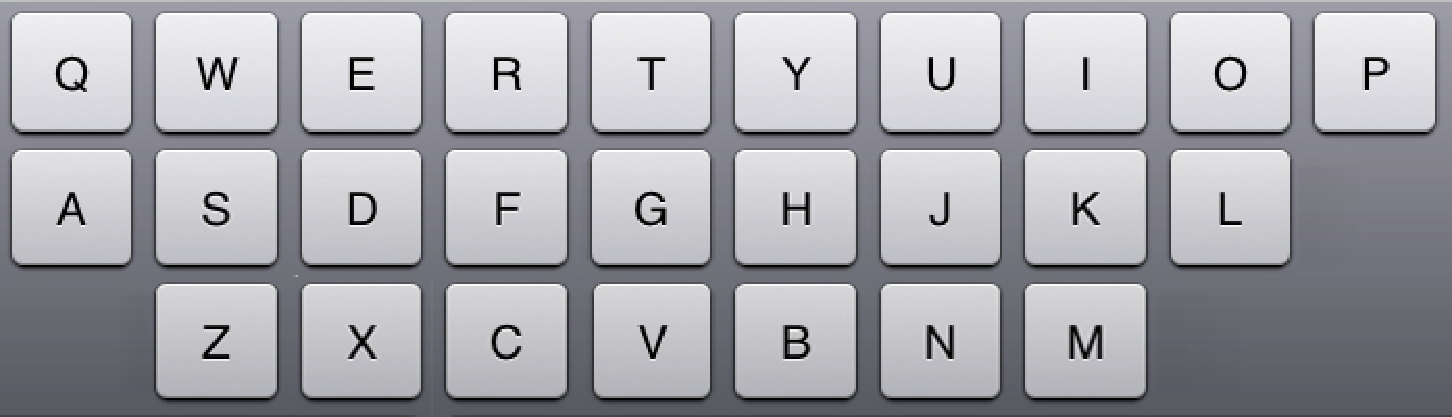
\includegraphics[width=.9\columnwidth]{figures/26Tap}

Layout and formatted exactly as regular mobile keyboard.
Aggressive autocorrect algorithm adjusted for typos and phonetic misspelling are applied.
The advantage of such keyboard is that the user does not need to change his interaction with a keyboard at all.
We noticed an unexpected phenomenon.
The user would  position their finger through gesture onto the desired key, but when they went to tap the key the lifting and lowering of the finger so that the proper key was not selected. 


\subsection{Design \#3 - 26-key Drag}
\vspace*{.1cm}
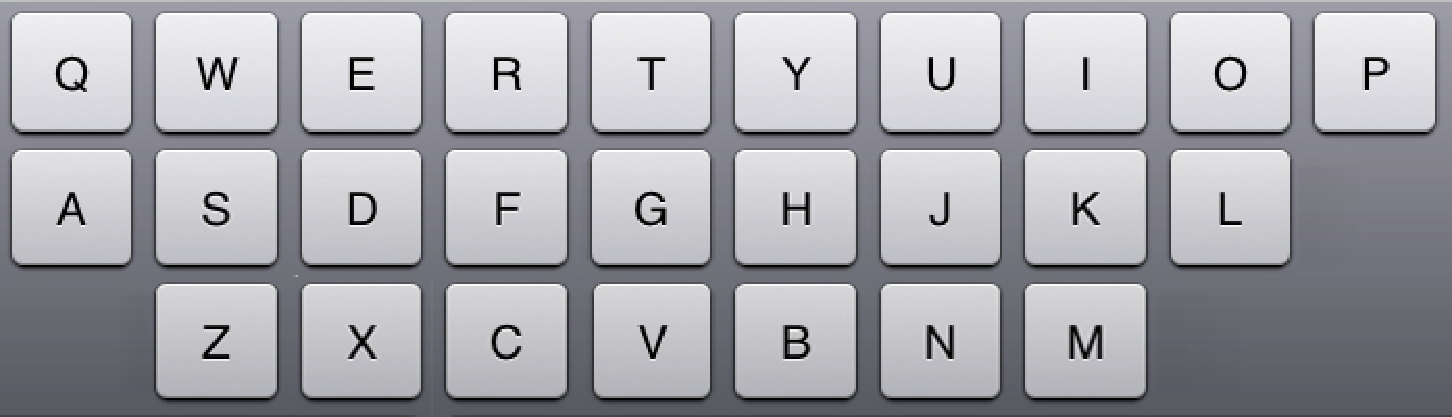
\includegraphics[width=.9\columnwidth]{figures/26Tap}

Similar to the 26-key tap, the layout of the mobile QWERTY keyboard is preserved, except tapping is replaced by dragging to specific keys.
Same autocorrect algorithm is applied


\subsection{Design \#4 - 8-key Drag}
\vspace*{.1cm}
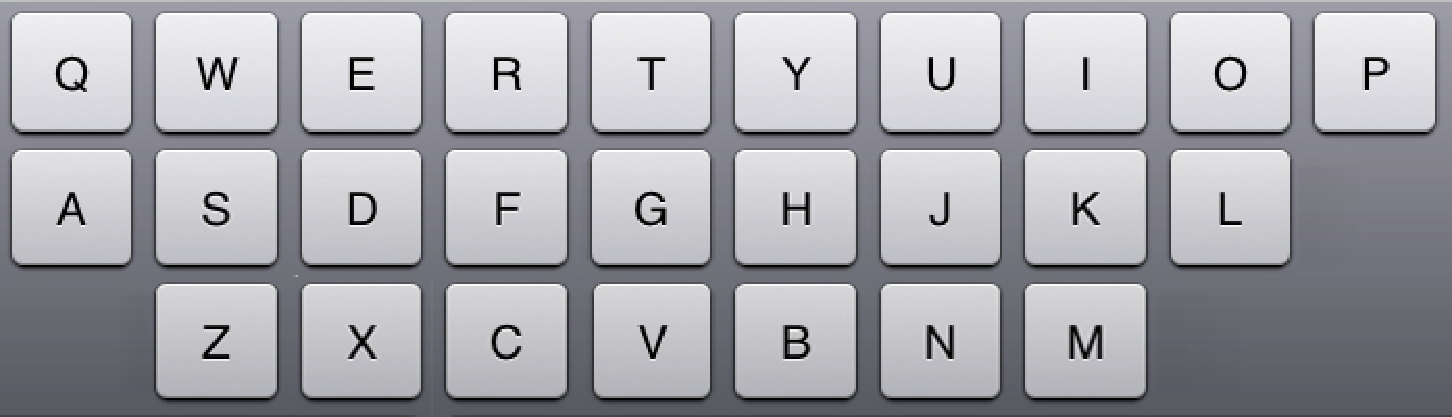
\includegraphics[width=.9\columnwidth]{figures/26Tap}

QWERTY keyboard is broken into 8 regions instead of 6.
User interact with this keyboard through dragging.
Both hands are required, with each hand dragging four directions (left, up, right, down) to input the 8 regions.

\subsection{Design \#5 - 6-key Tap}
\vspace*{.1cm}
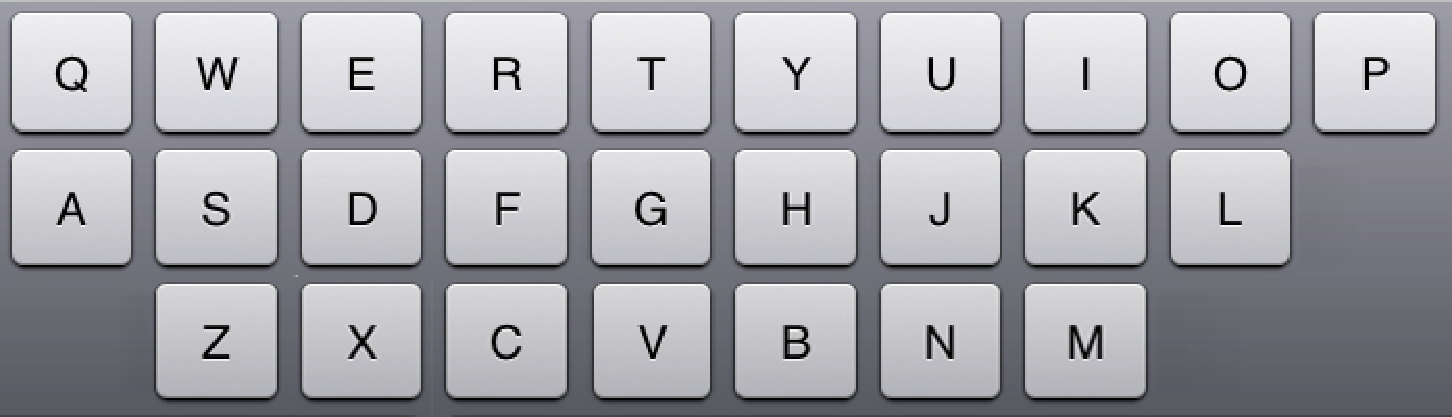
\includegraphics[width=.9\columnwidth]{figures/26Tap}

This is our first design utilizing batched keys. QWERTY keyboard is divided into 6 sections. Tapping corresponding regions triggers input for a whole section.
A word recommender algorithm in back end is required.


\subsection{Design \#6 - 6-key Drag}
\vspace*{.1cm}
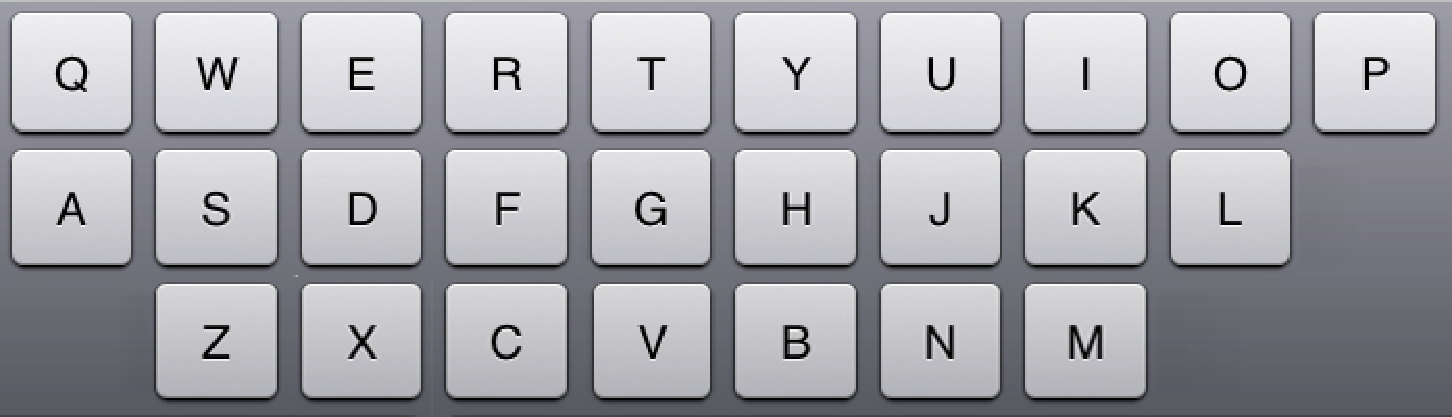
\includegraphics[width=.9\columnwidth]{figures/26Tap}

Similar to 6 keys tap, the method of interaction is changed to drag instead of tap.
A word recommender algorithm in back end is required.



\section{SwipeVR  Design Concepts}


Our design efforts focused on balancing three of the above factors: input speed, learning time, and physical size.
Our thinking was particularly influenced by the interaction design of cell phones that use T9 input, which relies on a database of words to disambiguate cell phone keypad keystrokes that are associated with more than one letter.
If we could design an input device that combined the best of the standard keyboard (fast text input, familiar layout) and the 12-key cell phone keypad (small size), we would have a device that could be used in off-the-desktop situations, potentially for extended typing tasks, with little degradation in performance. 

Despite the difficulties for the users to physically locate their finger outside of the virtual environment in order to interact with the keyboard on a mobile phone, the users are not completely helpless from their previous typing experience.
To start with, the users have muscle memory from typing on traditional mobile keyboards. With this previous experience, the user remembers, although imprecise, the location of letters if the layout of the keyboard is the same as what they are used to.

Thus, to leverage these previous knowledge of the users and address the problem that the users cannot physically see their fingers, we center our designs around two key features that we believe can help them adjust to typing in virtual reality: relative finger tracking, and batched keys.

\subsection{Relative Positioning}
Traditional mobile keyboard requires users to tap on the key precisely to enter an individual letter.
This method falls prey to specifically to the problem described above: users cannot tap on the individual keys accurate enough because they cannot see their finger relative to the touch screen of the mobile phone in a virtual environment.
Thus, we seek to use relative finger tracking to control a virtual cursor to solve the problem that users cannot see their hands.
Instead of having to be very precise about his finger positions, we instead rely on finger swiping or dragging to control a cursor in virtual reality.
Thus, users no longer need to consider the initial position of his finger because only the change in his finger position will be accounted for. 
Relative movement, instead of absolute movements, have also been found to be beneficial in reducing fatigue~\cite{Hincapie-Ramos:2014:CEM:2556288.2557130} so the user can start the interaction from their current position.

\subsection{Directional Swiping}
Even with relative finger tracking, typing in virtual reality still possesses the challenge that dragging to a specific key is slow and cumbersome given the limited screen space available for a mobile phone.
As users pick up the pace they are typing, their accuracy decreases for dragging precisely to individual letters.
To sustain the speed that they are typing in for each swipe requires considerable motion to complete with accuracy.
Thus, taking inspiration from traditional T9 keyboard widely used in feature phones, we arrive at a similar design choice of batching keys together to form sections that will register for all the keys in the section.
We group keys for efficiency(Hick's law)~\cite{card1983psychology}.

The advantages of such batched keys are two-fold.
Firstly, by batching some keys together, the user no longer need to be that precise in his dragging.
As long as he reaches within the proximity of the target letter, the whole region will register.
Secondly, by batching the keys together, we allow users to simply drag to direction of the key instead of having to take effort to get to the target letter, which drastically reduce the work a user has to do in a single swipe.




\begin{figure*}
  \centering
  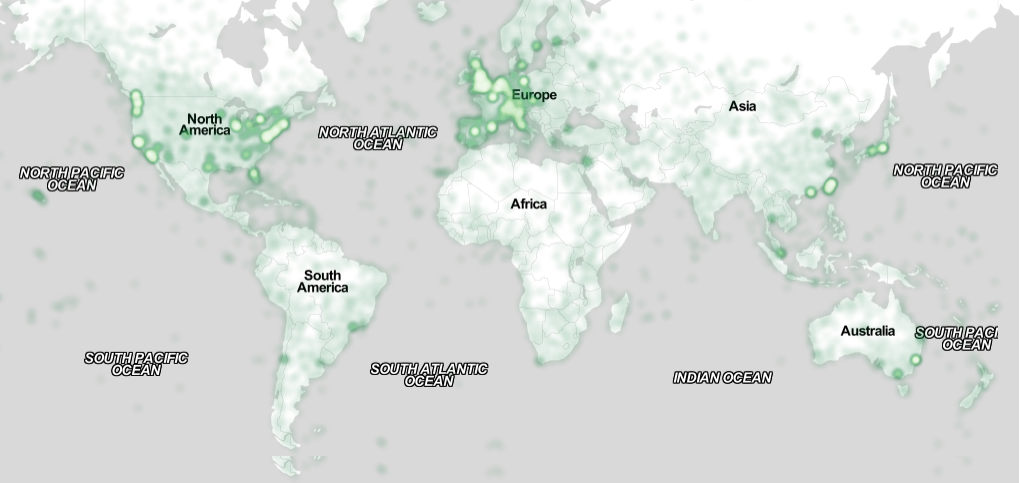
\includegraphics[width=1.75\columnwidth]{figures/map}
  \caption{Example of the system.  When the user want to type .}
  ~\label{fig:example}
\end{figure*}



\begin{figure}
\centering

  \begin{tikzpicture}

  \def \n {5}
  \def \radius {3cm}
  \def \margin {8} % margin in angles, depends on the radius

  \foreach \s in {1,...,\n}
  {
    \node[draw, circle] at ({360/\n * (\s - 1)}:\radius) {$\s$};
    \draw[->, >=latex] ({360/\n * (\s - 1)+\margin}:\radius) 
      arc ({360/\n * (\s - 1)+\margin}:{360/\n * (\s)-\margin}:\radius);
  	}
	\end{tikzpicture}

	\caption{
    Controller\\
	Intent Detection Classifier\\
    triager \\
	|swipe          |                |\\
    ngram           deterministic     \\
    selection        letter           \\
}~\label{fig:systemFlowchart}
\end{figure}


%\section{The SwipeVR Text Entry Technique}


This design is a special case of relative finger tracking in that it uses inspiration in Swype. 
The user draws a trail which is then translated to a series of taps on the 6 keys tap keyboard through finding the inflection points on the user's finger movement path.
We describe a specialized keyboard for text entry that maps six rows of a standard keyboard onto a virtual keyboard, shown in Figure~\ref{fig:swipeVRLayout}.
Different words are encoded via modifier keys and multi-swipe input with the thumb.
Use of the keyboard also relies on lexicon-based disambiguation.

\subsection{Slow and Fast Keyboard}
\subsection{Gesture Detection}
A special case of relative finger tracking is the 6 Keys Swype keyboard design.
This keyboard design resembles the use of Swype keyboard on Android.
In such a case, finger swipe data needs to be translated to a sequence of numbers to denote the chosen letters
We implement this functionality by finding the inflection points along the path (see Figure~\ref{fig:position}).
After a few experimental trials, we realized that as the user changes direction of his finger movement, the speed of his finger movement decreases (see Figure~\ref{fig:acceleration}).
Combining actual directional changes of the swipe trail, we are able to identify the inflection points. 

\subsection{Special Interactions}



Interaction with keyboards with relative finger tracking requires extra layers of complication by the nature of the swiping motion.
Special means of interaction such as space and delete becomes a none trivial task for the user would need to drag the virtual cursor to a designated location.
However, this form of interaction is against the motive of the finger tracking motion, which is to simplify users' interaction with the keyboard.
Thus, we designate new forms of interaction to help users use space and delete utility quickly.
Presses and hold on the trigger as shown in Figure~\ref{fig:trigger} to show a list of special keys, as shown in Figure~\ref{fig:specialCharacters}.


\subsection{Deterministic Inputs}
Measure for 0 acceleration as shown in Figure~\ref{fig:acceleration}.

\subsubsection{Delete}
For delete, users can double tap the mobile phone screen.

\subsubsection{Space}
To insert a space, the user clicks the trigger button on the bottom side of the controller, as shown in Figure~\ref{fig:trigger}. 
We experimented with automatically inserting a space after a certain timeout periods between 150 and 500ms.  However, we found that users prefered to have the control of when to insert the space themselves.




\subsubsection{Word option}
Long swipe


\begin{figure}
  \centering

  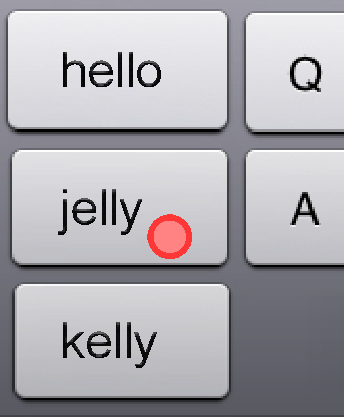
\includegraphics[width=.3\columnwidth]{figures/multiword}
  
  \caption{The Bayesian word recommender infers the most probable words with the same representation as the entered batched keys. In the above example, \textit{hello}, \textit{jelly}, and \textit{kelly} have the same representation, Key 5, 1, 5, 5, then 4. The algorithm uses 2-gram and 3-gram data from Google, part of speech frequency for English dictionary, word frequency for the entire English language, and produces a prediction score. The word with highest prediction score is the default output.  The user can \textit{long-swipe} to select alternate choices.}
  ~\label{fig:multiword}
\end{figure}


Another form of special interaction worth mentioning is choosing word options.
With batched keys, the word users input may contain uncertainty - multiple words with the same representation. See Figure~\ref{fig:multiword}.

Although the word recommender algorithm will produce the most likely word, it is not guaranteed such word is the choice of the users.
Thus, we enable users to choose among the next few most probable options.
The users simply drag towards the direction of the displayed option to choose the alternatives.

\subsection{Bayesian Word Recommender}
The Bayesian word recommender aims to infer the most probable words with the same representation in the same configuration of batched keys.
For instance, in 6 keys designs, word ``hello" and ``jelly" has the same representation ``51554".
This recommender algorithm use 2-gram and 3-gram data from Google Books Ngram Viewer\footnote{http://storage.googleapis.com/books/ngrams/books/datasetsv2.html}, part of speech frequency for English dictionary, individual word frequency for the entire English language, and produces a prediction score.
The word with highest prediction score will be selected as the most probable word.

\subsection{Implementation}
SwipeVR consists of three components: software for the controller , software for the virtual reality display, and a back end software.
The controller software (Android or HTC Vive) collects the finger movement from the users and relay the data to back end server.
The data relayed varies for different input methods.
For relative finger tracking, an unscaled change vector is emitted for every unit time interval to show the finger movement on screen, whereas absolute finger tracking, a pair of scaled coordinates are sent to show the position of the touch on the screen.
For designs with batched keys, a number indicating which key is selected is also emitted, whereas designs with 26 individual keys emits no additional information.
Selection of letter is determined based on the position of the cursor in virtual reality. (see Figure~\ref{fig:systemScreenshot})(see Figure~\ref{fig:systemFlowchart})

The back end server collects these finger movement data described above.
If the design uses batched keys, the inputted number sequence will go through a Bayesian algorithm that determines the most probable word with the same batched key combinations. The produced word is then sent to the virtual reality environment for display.
On the other hand, if no batched keys are used, finger position data will be directly sent to the virtual reality environment for display.



\begin{figure}
  \centering


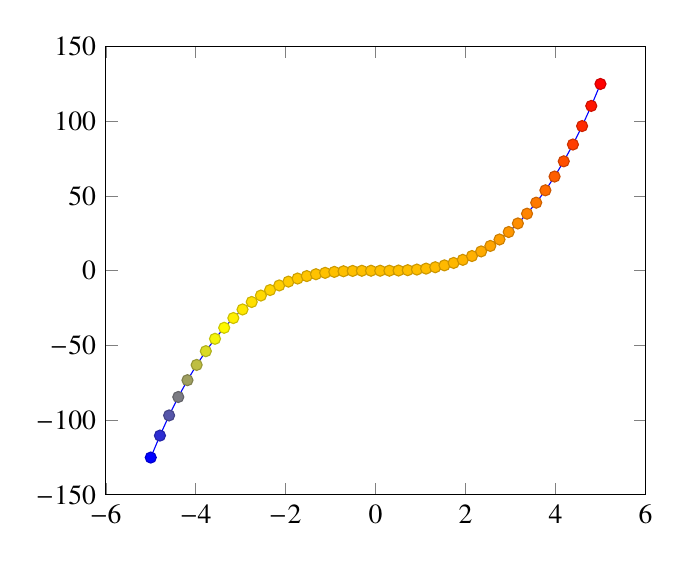
\begin{tikzpicture}
\begin{axis}
\addplot+[scatter,
samples=50,scatter src=y]
{x^3};
\end{axis}
\end{tikzpicture}
	\caption{Gesture detection graph with acceleration}~\label{fig:acceleration}
\end{figure}

\begin{figure}
\centering
  \begin{tikzpicture}
  \begin{axis}[
    xlabel=$x$,
    ylabel=$\sin(x)$
  ]
    \addplot gnuplot[id=sin]{sin(x)}; 
  \end{axis}
\end{tikzpicture}

  
  \caption{Gesture tracking graph with position}~\label{fig:position}
\end{figure}



\subsection{Overall Structure}
The system is composed of three parts: an Android client, a backend server and a virtual environment. The Android client parses finger movement to letters. In some cases, such as Swype with 6 keys, finger movement data are processed to groups numbers by an algorithm that takes acceleration and direction change of finger to find inflection points on the path.

\subsection{Client-side}
The Android client then relays user input to the backend where the input is passed through a Bayesian model, using dictionary word frequency, part of speech frequency, and Google NGram data Such model determines the most likely word, which is sent to the virtual environment for display.

\subsection{Visual interface design}
Designing effective visual interfaces is critical to the overall usability of the system. Here we present some of the key components of used in this regard. 

\subsubsection{Feedback and output interfaces}
\subsubsection{Managing Visual Attention 1}


\begin{figure}
  \centering
  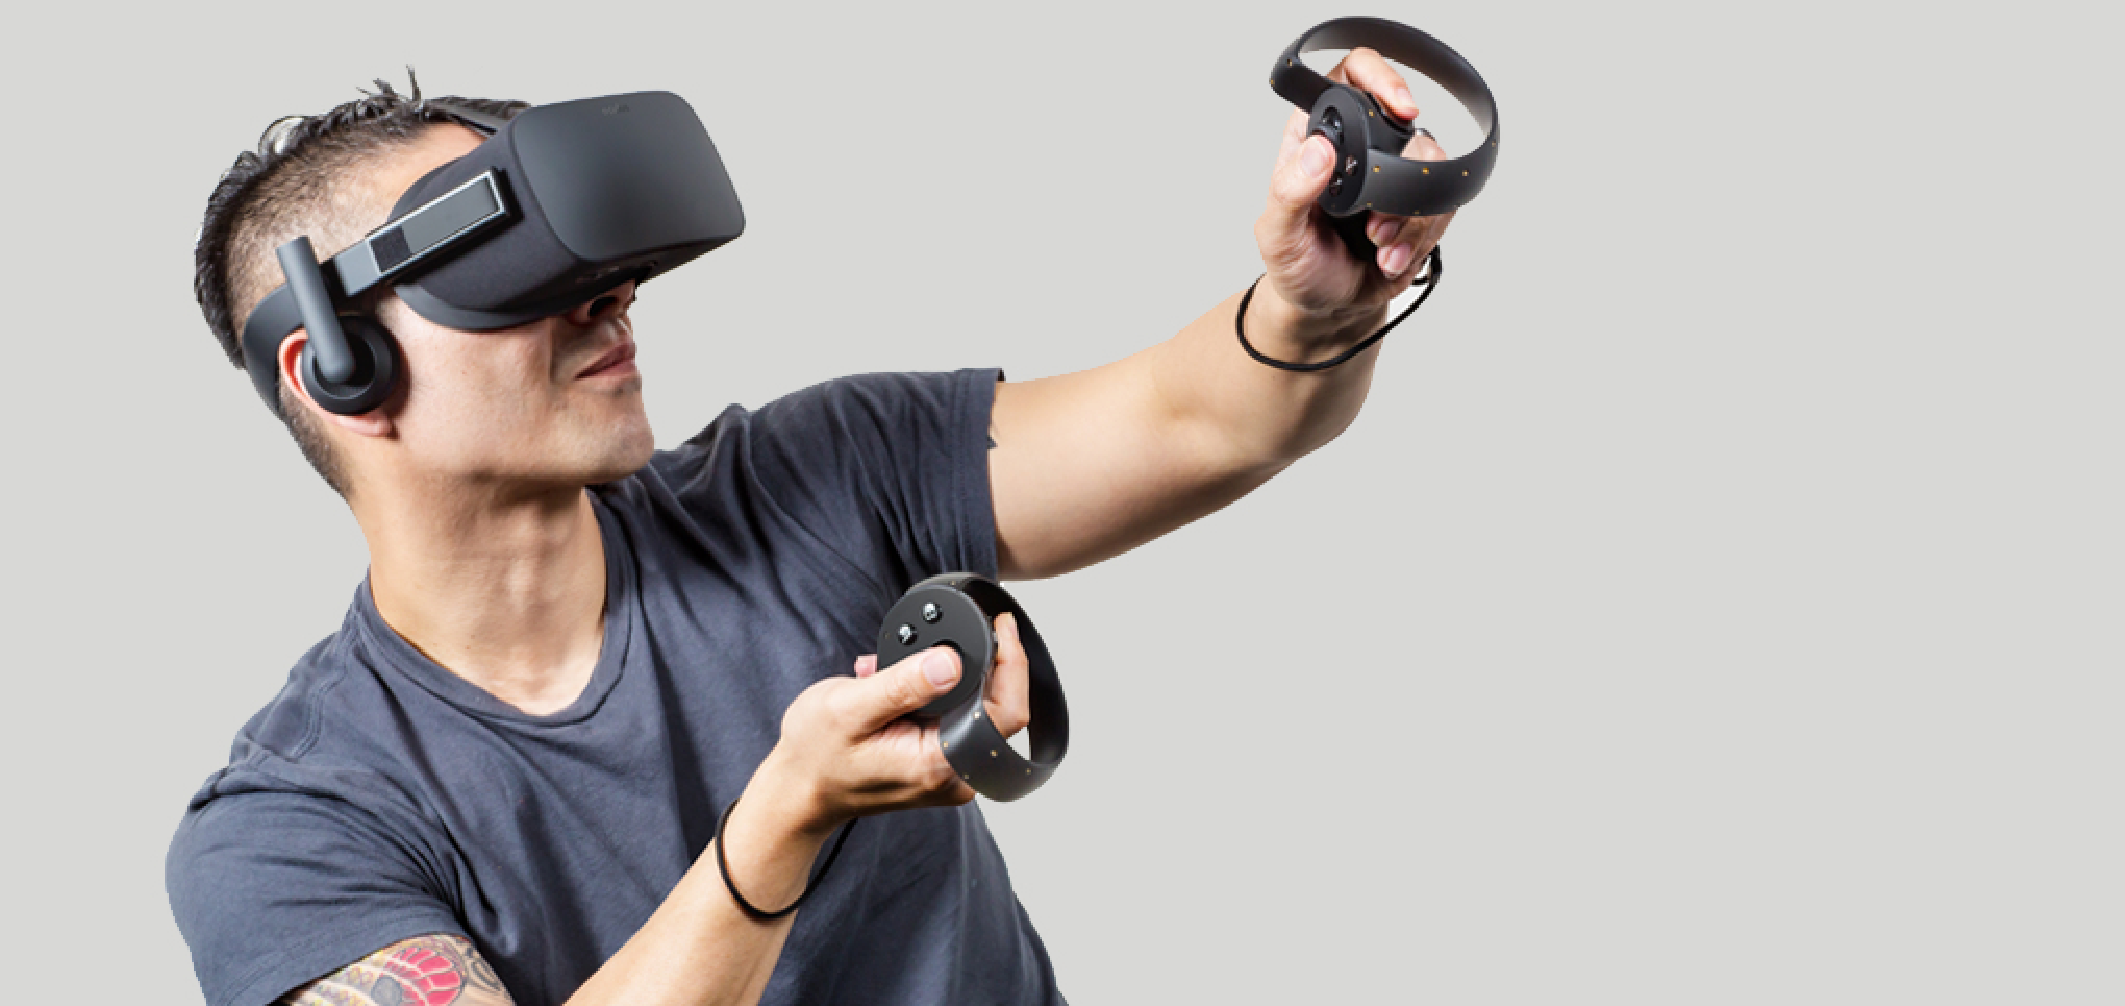
\includegraphics[width=1\columnwidth]{figures/manVR}
  \caption{User using SwipeVR.}~\label{fig:figure2}
\end{figure}


\begin{table}
  \centering
  \begin{tabular}{l r r r r}
    % \toprule
    & & \multicolumn{2}{c}{\small{\textbf{Test Conditions}}} \\
    \cmidrule(r){2-5}
    {\small\textit{Input}}
    & {\small \textit{Speech}}
    & {\small \textit{Mobile Keyboard}}
    & {\small \textit{Gaze}}
    & {\small \textit{SwipeVR}} \\
    \midrule
    Words per Minute & 152 & 52 & 9 & 49 \\
    Uncorrected Error Rate & 3\% & 3\% & 3\% & 3\% \\
    Corrected Error Rate & 3\% & 3\% & 3\% & 3\%\\
    Total Error Rate & 3\% & 3\% & 3\% & 3\%\\
    % \bottomrule
  \end{tabular}
  \caption{ Mean measures for the four input methods.}~\label{tab:tableResults}
\end{table}

\begin{figure}
\centering
\begin{tikzpicture}
\begin{axis}
\addplot+[ybar] plot coordinates
{(0,3) (1,2) (2,4) (3,1) (4,2)};
\end{axis}
\end{tikzpicture}

\caption{Words per minute as a function of language and input method.}~\label{fig:graphWPM}
\end{figure}

\begin{figure}
\centering

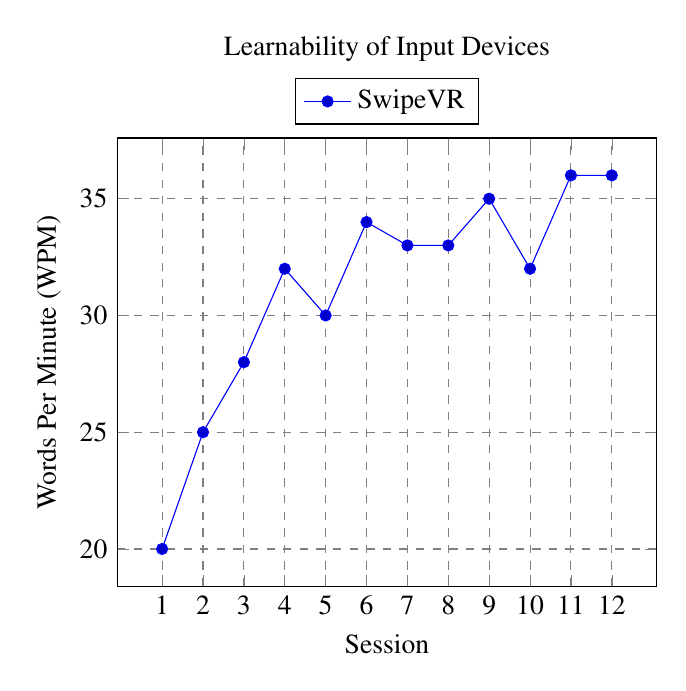
\begin{tikzpicture}
\pgfplotsset{
		every axis legend/.append style={
			at={(0.5,1.03)
		},
		anchor=south
    }
}
\pgfplotsset{grid style={dashed,gray}}
%\pgfplotsset{minor grid style={dashed,red}}
%\pgfplotsset{major grid style={dotted,green!50!black}}

\begin{axis}[
legend columns=-1,
xlabel=Session,
ylabel=Words Per Minute (WPM),
 title style={at={(0.5,0)},anchor=south,yshift=180},
 title = Learnability of Input Devices,
 %ytick={0,5,10,15,20},
 %minor ytick={1,2,3,4,5,6,7,8,9,10,11,12,13,14,15,16,17,18,19,20},
 xtick={1,2,3,4,5,6,7,8,9,10,11,12},
 %minor xtick={1,2,3,4,5,6,7,8,9,10,11,12,13,14,15,16,17,18,19,20},
 grid=both,
]
\addplot coordinates
{
	(1,20)(2,25)(3,28)(4,32)(5,30)(6,34)(7,33)(8,33)(9,35)(10,32)(11,36)(12,36)
};

\legend{SwipeVR, Speech, Gaze, Mobile}

\end{axis}
\end{tikzpicture}

%4.7.1 Markers for graph fixing the circle, square, x, triangle overloading

\caption{
Graph of learnability for each of the input methods.
Learning curves for the four tested entry methods.
Entry rate on each block of 20 sentences in the second pilot.
Each line is a single participant.
}~\label{fig:learnability}
\end{figure}



\section{Evaluation}
We performed a within-subject user study to evaluate performance and user experience of SwiepVR.
We measure text entry performance by means of words per minute (WPM) rate and uncorrected word error rate (WER) (cf. [5]). UX was evaluated using the usability
questionnaires UEQ [12] and SUS [4] and some self-made items.


\subsection{Hypotheses}
We formulated three hypotheses.

\subsubsection{Hypothesis 1}
The uncorrected error rate to enter text using SwipeVR in virtual reality will be within 20\% of entering text on a smart phone keyboard in reality.

\subsubsection{Hypothesis 2}
More time is spent error correcting and editing than entering text.  Input mechanism should take this into account.

\subsubsection{Hypothesis 3}
SwipeVR is faster at editing and error correcting than smart phone keyboard in reality.

%\subsubsection{Hypothesis 4}
%Something about using multiple input mechanisms that don't conflict with each other. Error correction will not overlap in bandwidth with text entry.

We think that \textit{Hypothesis 1} will

We think that \textit{Hypothesis 2} will

We think that \textit{Hypothesis 3} holds as SwipeVR offers a tighter integrated between input devices and output displays used in smart phones.
The controllers in virtual reality are more \textit{expressive}~\cite{card1990design} than mobile phone keyboards.

\subsection{Participants}
Fifteen subjects (5 female) participated in the study.
Each subject took about 30 minutes to complete the study.

\subsection{Phrase Set}
We selected fifty phrases from a collection of five-hundred phrases commonly used for text entry evaluations~\cite{mackenzie2003phrase}.
To allow for cross-comparison to other text entry methods, the corpus doesn't include phrases with punctuation marks.
Non-alphanumeric symbols are rarely considered in text input research~\cite{mackenzie2003phrase} even though some punctuations (. - ' ( ) ") are more frequent than the least common English letter (q)~\cite{malikpunctuation}.
 
SwipeVR allows for the entry of non-alphanumeric symbols using a different interaction technique for words then for punctuation and characters.
To measure the  we add to the phrase set ten phrases for the user to enter that contain non-alphanumeric symbols.
We add five phrases with punctuation marks so the evaluation more closely mimics real-life interactions.
This addition more fully tests the transition time between interaction techniques. 

Copying pre-selected phrase is usually the preferred method for text entry when doing evaluations in a lab setting~\cite{mackenzie2002character, mackenzie2003phrase}.
Although, copying pre-selected entry rates should be regarded differently from true, ``in the wild'' results when the user is composing text instead of transcribing prompted phrases.
In particular, reading a pre-selected phrase has a noticalbly different cadence and certainty that is typically not present in natural voice interactions which leads to what we hypothesize could be an optimistic measurement of voice input.

When the user composes text on their own, there could be substantial thinking time ~\cite{shneiderman2000limits} and other considerations that are difficult to measure.
We only use pre-selected phrases and rely on qualitative feedback to develop a holistic understanding for usability.

\subsection{Procedure}
Participants entered a series of phrases from the phrase set.
One of our metrics is the learnability of the system so we don't give users practice trials before beginning the actual test.

For each user we conduct twelve sequential sessions.
In each session, a user enters six phrases.
After entering all the phrases with both input methods, the participant filled out
a questionnaire regarding their quantitative feedback on the text entry method.
Finally, subjects were asked for additional comments.

\subsection{Measures}
In the field of text entry, several metrics are used to characterize a method's performance ~\cite{wobbrock2007measures,arif2009analysis}.
Here, we discuss the performance metrics we use to evaluate the performance of the input device.  

\subsubsection{Words per Minute}
Words per minute (~$WPM$) is perhaps the most widely reported empirical measure of
text entry performance~\cite{wobbrock2007measures}:

\[ 
WPM={\vert T\vert -1\over S}\times 60\times{1\over 5}. \eqno{\hbox{(1)}}
\]

Where, $S$ is the time in seconds from the first key press to the last, which means that the entry of the first character is never timed, which is the motivation for the "- 1" in the numerator of (1)~\cite{yamada1980historical}.
English words by convention are treated as having five characters~\cite{yamada1980historical}.

\subsubsection{Error Rate}
Error Rate (~$ER$) is the ratio of the total number of incorrect characters in the transcribed text to the length of the transcribed text:

\[
ER={INF\over \vert T\vert }\times 100\%. \eqno{\hbox{(2)}}
\]

Where, Incorrect Not Fixed (~$INF$) is the number of unnoticed incorrect characters in the transcribed text.


\begin{table}\centering
\ra{1.3}
\begin{tabular}{@{}rrrrr@{}}\toprule
            &             & $SwipeVR$  \\
\midrule
$Positioning$     &             & relative        \\

%    Correction Method    & X       & X       & X       &   \checkmark    \\ 

\bottomrule
\end{tabular}
\caption{Ontology of input methods.}
\label{table:usability}
\end{table}


\subsubsection{Subjective }
we ask the user to evaluate each entry mechanism on a 5-point Likert Scale (Strongly Disagree, Disagree, neutral, Agree, Strongly Agree).
Additionally, users are  interviewed to further understand the their qualitative experience.

\subsubsection{Performance}
The input device felt responsive\\
The visuals were smooth and didn't freeze\\
The input device worked properly\\
The system was over responsive and showed inputs that I didn't enter\\
The system was under responsive and didn't showed inputs that I thought I entered

\subsubsection{Design}
It is easy to understand what to do with the input device\\
It was easy to learn how to use the input device\\
The interface was intuitive\\
This application has a graphical interface pleasant and understandable\\
The text and input were clearly visible

\subsubsection{Ergonomics}
I felt arm strain\\
I felt hand strain\\
I felt hand Nausea\\
I felt dizzy when using the system\\
I felt nauseous when using the system

\subsubsection{Applications}
I would use the input device to do a web search\\
I would use the input device to write an email\\
I would use the input device in public\\
I would use the input device at home\\
I would use the input device at a park\\
I would use the input device to chat (text)\\
I would use the input device to edit a letter

\section{Results}
\subsection{Word Per Minute}
The average rate for text entry was 34 WPM.  

\subsection{Error Rate}
The average error rate for text entry was 4\%.  

\begin{figure}
\centering

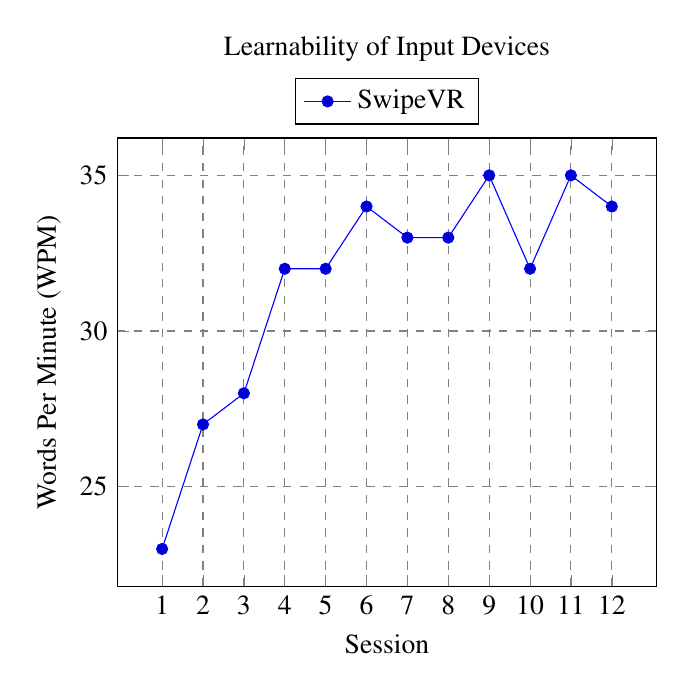
\begin{tikzpicture}
\pgfplotsset{
    every axis legend/.append style={
      at={(0.5,1.03)
    },
    anchor=south
    }
}
\pgfplotsset{grid style={dashed,gray}}
%\pgfplotsset{minor grid style={dashed,red}}
%\pgfplotsset{major grid style={dotted,green!50!black}}

\begin{axis}[
legend columns=-1,
xlabel=Session,
ylabel=Words Per Minute (WPM),
 title style={at={(0.5,0)},anchor=south,yshift=180},
 title = Learnability of Input Devices,
 %ytick={0,5,10,15,20},
 %minor ytick={1,2,3,4,5,6,7,8,9,10,11,12,13,14,15,16,17,18,19,20},
 xtick={1,2,3,4,5,6,7,8,9,10,11,12},
 %minor xtick={1,2,3,4,5,6,7,8,9,10,11,12,13,14,15,16,17,18,19,20},
 grid=both,
]
\addplot coordinates
{
  (1,23)(2,27)(3,28)(4,32)(5,32)(6,34)(7,33)(8,33)(9,35)(10,32)(11,35)(12,34)
};

\legend{SwipeVR, Speech, Gaze, Mobile}

\end{axis}
\end{tikzpicture}

%4.7.1 Markers for graph fixing the circle, square, x, triangle overloading

\caption{
Graph of learnability for each of the input methods.
Learning curves for the four tested entry methods.
Entry rate on each block of 20 sentences in the second pilot.
Each line is a single participant.
}~\label{fig:learnability}
\end{figure}


\subsection{Learnability}
The extrapolated learning curve is shown in Figure~\ref{fig:learnability}.
A curve is fit according to a power law and allow us to speculate about performance in future sessions.

\subsection{Usability}
We found that the 

\begin{figure}
\centering
  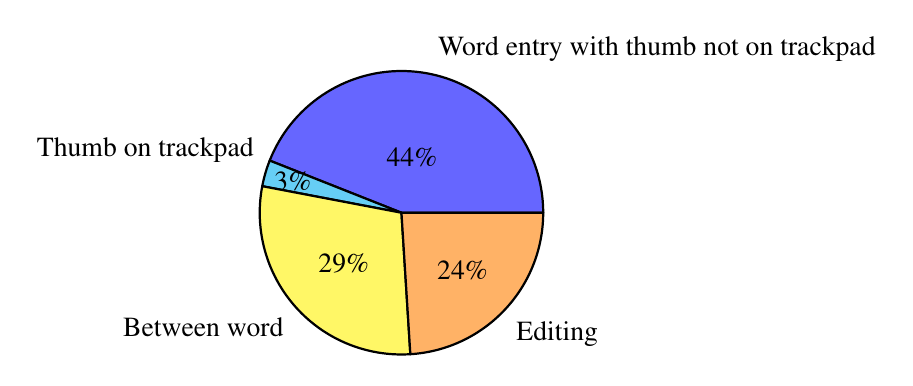
\begin{tikzpicture}[scale=.6]

      \pie{44/Word entry with thumb not on trackpad, 3/Thumb on trackpad, 29/Between word, 24/Editing}[explode=0.1]
  \end{tikzpicture}
  \caption{The majority of time the user was entering a word, their thumb was not on the trackpad.  There was also a delay between when the user was entering words.
    }
  ~\label{fig:distance}
  \end{figure}

\begin{figure}
\centering
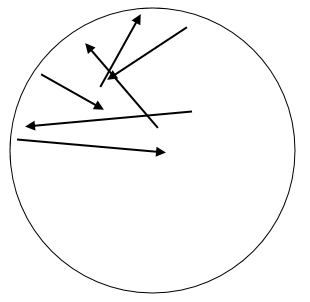
\includegraphics[width=0.5\columnwidth]{figures/circle}
  \caption{Sample of a right-handed users's swipes.  Most of the swipes are concetrated in the upper-left quadrant of the circluar trackpad.}

\label{fig:circle}

\end{figure}

\begin{figure}
\centering
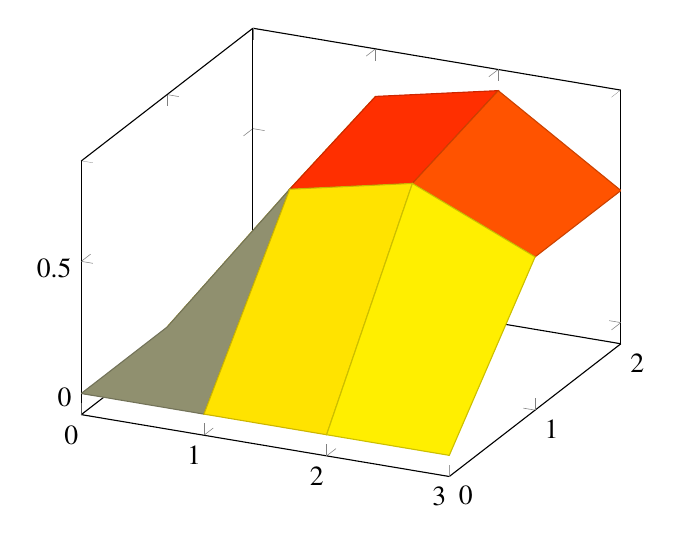
\begin{tikzpicture}
\begin{axis}
% this yields also a 3x4 matrix:
\addplot3[surf,mesh/rows=3] coordinates {
(0,0,0) (1,0,0) (2,0,0) (3,0,0)
(0,1,0) (1,1,0.6) (2,1,0.7) (3,1,0.5)
(0,2,0) (1,2,0.7) (2,2,0.8) (3,2,0.5)
};
\end{axis}
\end{tikzpicture}


  \caption{(Bar graph of arm strain, hand strain, neck strain, dizziness/nausea)  Differences between the initial and final subjective comfort ratings for each of the four techniques in the experiment 
}~\label{fig:graphLearning}
\end{figure}

\begin{figure}
\centering

  
\includegraphics[width=0.9\columnwidth]{figures/sigchi-logo}

  \caption{(Participants' subjective evaluation of difficulty 
}~\label{fig:graphLikert}
\end{figure}

\section{Discussion}
We argue that we have confirmed H1, H2, and H3.

Concerning H1 (SwipeVR faster than gaze), we find there are significant differences between text entry rates of both approaches.


\section{Future Work}
\subsection{Editing of text}
Most skilled manual activities involve two hands playing different roles ~\cite{guiard1987asymmetric, Casalta:1999:ETI:632716.632862}.
The two hands cooperate with one another as if they were assembled in series, thereby forming a kinematic chain.

More work has to be done, but for some tasks, such as, such as navigating and editing a document, it could be possible that This theory fits ell with the SwipeVR input controller.

Whilst the dominant hand is entering words, the non-dominant hand can be navigating the dominant to set the position in the document.
This could be done in one fluid task without having to clutch into a different input mode.

This is in  comparison to the typical setup whereby the user remove there dominant hand from the keyboard to reach for the mouse, navigate to the correct place in the document, then place there dominant and back on the keyboard. 
Meanwhile the non-dominant remains still

\subsection{Flexion and Extension of the Wrist}
The flexion and extension of the wrist~\cite{sarrafian1977study} is a high bandwidth bus, ~\cite{TBD}, almost as much as a finger, for information entry from the physical world into the virtual.
SwipeVR does not use this channel.
For example, the user could use the trigger button along with the wrist to select and move text around the document.
Again, while the dominant hand does the selecting, the non-dominant hand can reposition document or virtual world.


\section{Conclusion}

\subsection{Overcomes Latency and Proprioception with Swipe}
The lack of proproception in virtual reality is compounded by the latency.
For a user to be able to steer their finger to a key, the time needed to transmit information from the real to virtual and back to the ``real" through the  screen and into the eyes of the user is too long.

Therefore, we have to devices an alternate method of input that is not dependent on a feedback loop that requires the user to reach an absolute position on a keyboard.
Other input commonly used methods, such as gesture keyboard are subject to the same problem.

We device an alternate method that is only dependent on relative movement.
The user makes a swipe to one of six keys.
This reframes the domain of text input from a closed  feedback control problem to an open feedback control problem.
As such we are able to create a system for users that is able to efficiently enter text in virtual reality.


\subsection{Smooth Transition From Newbie to Novice to Expert }

A smooth pathway learnability is an important factor for an input device to gain widespread adoptability~\cite{}.
Some users will immediately reject an input device that requires too much upfront practice before it becomes useful.

SwipeVR offers a clear path from newbie to novice to expert. Newbie users are able to being using the system quickly by looking at the controller and slowly moving their thumb to a key.
As shown in the learnability chart, SwipeVR is instantly usable.
Novice users are able to periodically glance down or hold at the controller up within their field of view if they forget the position of a key.
Expert users are able to use memory to remember which way to move their thumb.
After some practice it becomes natural to memorize the location of the key by position.
At this point, the user is able to type, without looking down at the input device.
SwipeVR has a natural path to transition novice (low threshold) to expert (high ceiling) users~\cite{grover2013computational}.

\subsection{General Purpose Text Entry}
We hypothesize that virtual reality will be a general computing device much like the desktop or mobile phone.
While many of the apps in virtual reality will have their own specialized mechanism, we predict that at the operating system layer, there will be one general purpose text entry system that will be used across and only have to be learned how to use once.

This text entry system will need to be able to accommodate proper nouns, abbreviations, capital letters, colloquialism, passwords and other types of non-deterministic input.

SwipeVR is positioned well to accomodate these wide range of inputs and be the keyboard for a virtual reality operating system.

\subsection{Accessibility}
Virtual reality gives access access to something that they might never see in real life.
But for a disabled person, virtual reality might be the path to inclusion.
SwipeVR can be adapted for assistive technology products such as wands, joysticks, trackballs, touch screens.


\subsection{End}

concluding notes
\\
We present a fast text entry input device for virtual reality.
It is faster than the state of the art.
It can be used in public.
It dosnt tire your arms or vocal chords.

Using virtual reality for programming is a rich area for further discovery.
The large workspace that virtual reality provides is received well by users.

They keyboard is currently the weak point in many virtual reality applications.

Touch-typing on the keyboard is difficult as is switching context between the virtual reality controllers and the keyboard.

In the future, high-quality virtual reality headsets will be standalone devices, not tethered to desktop computers \cite{schaller1997moore}.
As the price of headsets decrease \cite{brown2016virtual}, virtual reality is positioned to become a democratizing technology.
Thus it is a worthwhile endeavour to determine how to program in virtual reality, both as a teaching tool for novices and as a more expressive tool for experts.





% Use a numbered list of references at the end of the article, ordered
% alphabetically by first author, and referenced by numbers in
% brackets~\cite{ethics, Klemmer:2002:WSC:503376.503378,
%   Mather:2000:MUT, Zellweger:2001:FAO:504216.504224}. For papers from
% conference proceedings, include the title of the paper and an
% abbreviated name of the conference (e.g., for Interact 2003
% proceedings, use \textit{Proc. Interact 2003}). Do not include the
% location of the conference or the exact date; do include the page
% numbers if available. See the examples of citations at the end of this
% document. Within this template file, use the \texttt{References} style
% for the text of your citation.

% Your references should be published materials accessible to the
% public.  Internal technical reports may be cited only if they are
% easily accessible (i.e., you provide the address for obtaining the
% report within your citation) and may be obtained by any reader for a
% nominal fee.  Proprietary information may not be cited. Private
% communications should be acknowledged in the main text, not referenced
% (e.g., ``[Robertson, personal communication]'').







% Balancing columns in a ref list is a bit of a pain because you
% either use a hack like flushend or balance, or manually insert
% a column break.  http://www.tex.ac.uk/cgi-bin/texfaq2html?label=balance
% multicols doesn't work because we're already in two-column mode,
% and flushend isn't awesome, so I choose balance.  See this
% for more info: http://cs.brown.edu/system/software/latex/doc/balance.pdf
%
% Note that in a perfect world balance wants to be in the first
% column of the last page.
%
% If balance doesn't work for you, you can remove that and
% hard-code a column break into the bbl file right before you
% submit:
%
% http://stackoverflow.com/questions/2149854/how-to-manually-equalize-columns-
% in-an-ieee-paper-if-using-bibtex
%
% Or, just remove \balance and give up on balancing the last page.
%
\balance{}


% REFERENCES FORMAT
% References must be the same font size as other body text.
\bibliographystyle{SIGCHI-Reference-Format}
\bibliography{sample}

\end{document}

%%% Local Variables:
%%% mode: latex
%%% TeX-master: t
%%% End:
